\section{Clustering and Robustness Results}
\label{sec:results}

\subsection{Confirmatory Matched-Backbone Performance}

All \FormalRunCount{} primary runs completed under one frozen source,
environment, and orchestration identity, with no failed tasks.  We report
dataset-level seed averages and retain every prespecified dataset, variant, and
seed.  Table~\ref{tab:confirmatory_overall}, Figure~\ref{fig:confirmatory}, and the following contrast
sentences are generated directly from the checksum-verified run master.

\begin{table}[t]
\centering
\caption{Matched-backbone confirmatory performance. Values are means across dataset-level seed averages; dispersion is the standard deviation across datasets.}
\label{tab:confirmatory_overall}
\begin{tabular}{lccc}
\toprule
Method & ARI & NMI & Macro-F1 \\
\midrule
NoMix & 0.611 (0.277) & 0.725 (0.185) & 0.612 (0.167) \\
RandomMix & 0.594 (0.289) & 0.716 (0.188) & 0.583 (0.151) \\
scVICAR-F & 0.609 (0.279) & 0.727 (0.179) & 0.616 (0.162) \\
T-Edge & 0.606 (0.283) & 0.727 (0.180) & 0.603 (0.175) \\
T-Gate & 0.621 (0.295) & 0.725 (0.189) & 0.605 (0.141) \\
scVICAR-T & 0.617 (0.283) & 0.725 (0.185) & 0.600 (0.136) \\
\bottomrule
\end{tabular}
\end{table}


scVICAR-F versus NoMix yielded a mean paired ARI difference of -0.002 (dataset bootstrap 95\% CI -0.005 to 0.001; wins/ties/losses 1/0/5; Holm-adjusted permutation p=0.6923).

scVICAR-T versus NoMix yielded a mean paired ARI difference of 0.005 (dataset bootstrap 95\% CI -0.027 to 0.042; wins/ties/losses 3/0/3; Holm-adjusted permutation p=1.0000).

scVICAR-T versus scVICAR-F yielded a mean paired ARI difference of 0.008 (dataset bootstrap 95\% CI -0.028 to 0.047; wins/ties/losses 3/0/3; Holm-adjusted permutation p=1.0000). The latter is a clean-graph comparison and is not interpreted as a requirement that topology adaptation dominate on every dataset.


\begin{figure*}[t]
  \centering
  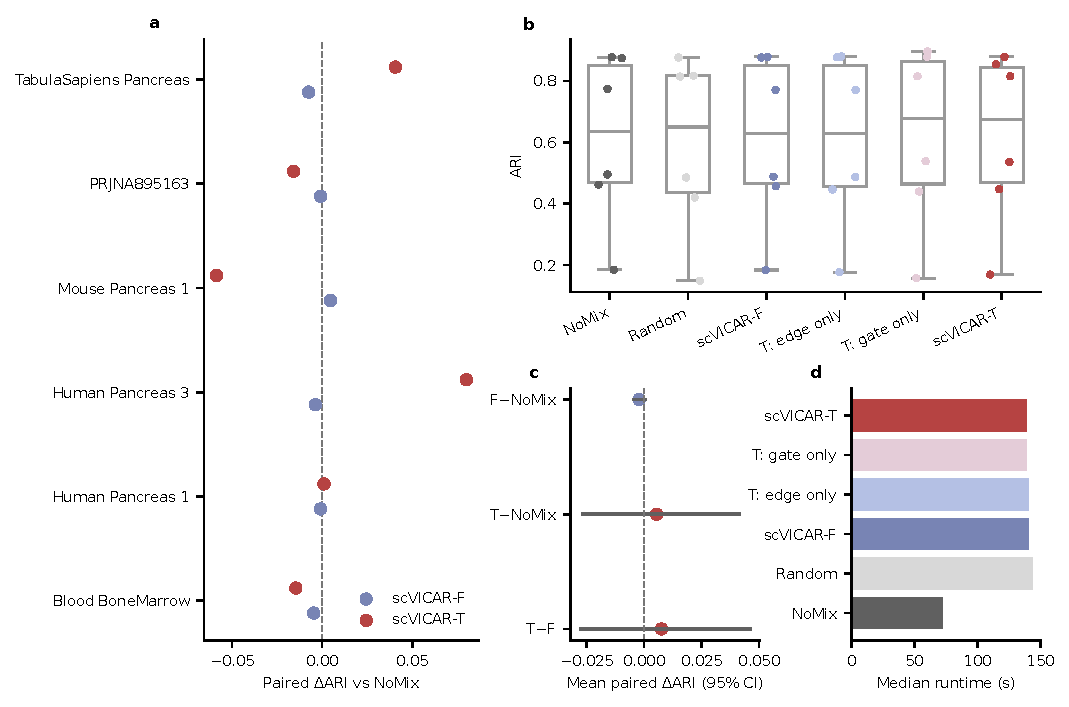
\includegraphics[width=\textwidth]{../figures/final/fig2_confirmatory.pdf}
  \caption{Confirmatory matched-backbone results across six held-out datasets
  and all three model seeds. (a) Dataset-level paired ARI changes relative to
  NoMix. (b) ARI distributions for all six matched variants. (c) Prespecified
  paired effects with dataset-level 95\% confidence intervals. (d) Median
  runtime under the common training budget. No best seed or dataset is
  selected.}
  \label{fig:confirmatory}
\end{figure*}

The confirmatory clean-graph data therefore do not support a general ARI
advantage for fixed vicinal recovery.  scVICAR-F improved on one dataset and
decreased ARI on five, although the mean effect was small.  The full adaptive
variant was heterogeneous: it improved markedly on Human Pancreas 3 and more
moderately on Tabula Sapiens Pancreas, while decreasing ARI on Mouse Pancreas 1,
PRJNA895163, and Blood--Bone Marrow.  Its positive mean T--NoMix effect was not
distinguishable from zero at the dataset level.  We consequently treat the
clean analysis as evidence of dataset dependence and reserve the principal
topology claim for the prespecified contamination experiment.

\subsection{External Baselines}

\begin{table*}[t]
\centering
\caption{External baselines and principal matched variants. Values are means (SD) across six dataset-level seed averages. scDCC, scDeepCluster, and scRCL use known $K$ during their published clustering-oriented training; other rows use $K$ only for post-hoc KMeans.}
\label{tab:external_baselines}
\begin{tabular}{lrrrr}
\toprule
Method & ARI & NMI & Macro-F1 & Runtime (s) \\ 
\midrule
PCA+KMeans & 0.587 (0.244) & 0.693 (0.197) & 0.549 (0.151) & 16.5 (7.5) \\
Original scMAE & 0.604 (0.282) & 0.724 (0.180) & 0.605 (0.174) & 84.7 (82.7) \\
scVI & 0.428 (0.149) & 0.669 (0.141) & 0.509 (0.101) & 289.9 (326.8) \\
scDCC & 0.555 (0.212) & 0.718 (0.146) & 0.556 (0.130) & 859.0 (1006.1) \\
scDeepCluster & 0.508 (0.193) & 0.688 (0.138) & 0.542 (0.145) & 1022.6 (1214.6) \\
scRCL & 0.524 (0.227) & 0.700 (0.165) & 0.511 (0.156) & 150.1 (152.6) \\
Matched NoMix & 0.611 (0.277) & 0.725 (0.185) & 0.612 (0.167) & 94.1 (98.4) \\
scVICAR-F & 0.609 (0.279) & 0.727 (0.179) & 0.616 (0.162) & 190.7 (218.5) \\
scVICAR-T & 0.617 (0.283) & 0.725 (0.185) & 0.600 (0.136) & 191.1 (219.5) \\
\bottomrule
\end{tabular}
\end{table*}

External methods are reported under their frozen published adapters. Every row averages all three seeds within each dataset before the six-dataset summary. scVICAR-T had the highest mean ARI (0.617), 2.13\% above Original scMAE (0.604); scVICAR-F had the highest mean NMI (0.727) and macro-F1 (0.616). Matched NoMix reached 0.611 ARI. The matched-variant analysis estimates the contribution of vicinal mixing. Wall-clock times are descriptive because CPU/GPU frameworks and interpreters differ across published implementations.


\subsection{Component and Negative-Control Ablations}

Random mixing produced the lowest descriptive mean ARI (0.594), below NoMix
(0.611), arguing against a generic smoothing explanation.  Edge-only weighting
also did not improve the mean (0.606).  The gate-only variant had the highest
descriptive mean ARI (0.621), followed by the full model (0.617), but both
retained substantial between-dataset variation.  Because gate-only versus
NoMix was not one of the three confirmatory inferential contrasts, this pattern
is treated as component evidence rather than a new significance claim.  The
matched design attributes these descriptive differences to corruption
construction rather than model capacity.  Vicinal variants required roughly
twice the mean runtime of NoMix in this implementation.
Figure~\ref{fig:components} shows the corresponding matched component and
representation-geometry summaries without adding post-hoc inferential tests.

\begin{figure*}[t]
  \centering
  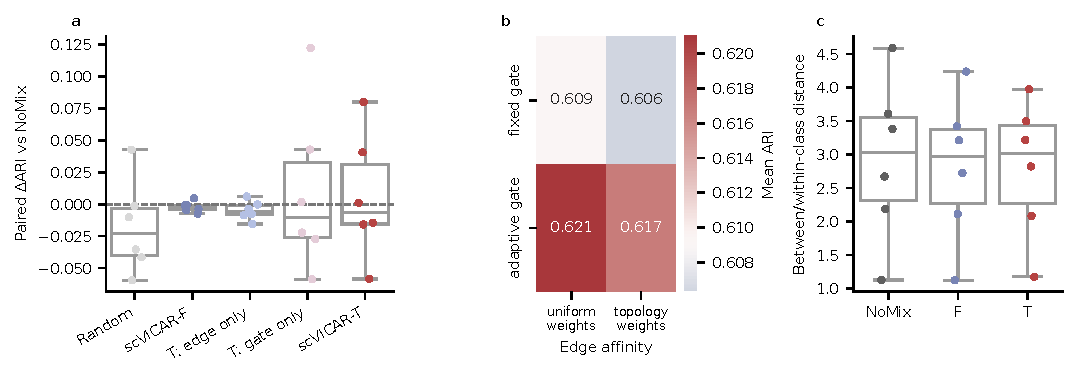
\includegraphics[width=\textwidth]{../figures/final/fig3_components.pdf}
  \caption{Matched component and negative-control evidence. Random mixing,
  fixed vicinal corruption, topology edge weighting, topology gating, and the
  full adaptive model are compared without changing the backbone or budget.
  The descriptive gate-only pattern is not promoted to a post-hoc confirmatory
  hypothesis.}
  \label{fig:components}
\end{figure*}

\subsection{Fixed-Resolution Leiden Sensitivity Analysis}

\begin{table}[t]
\centering
\caption{Fixed-resolution Leiden sensitivity analysis. Values are means (SD) across the six dataset-level seed averages; resolution is 1.0 and is never label-tuned.}
\label{tab:leiden_overall}
\begin{tabular}{lccc}
\toprule
Method & ARI & NMI & Macro-F1 \\ 
\midrule
NoMix & 0.335 (0.093) & 0.648 (0.099) & 0.587 (0.123) \\
RandomMix & 0.361 (0.122) & 0.658 (0.109) & 0.593 (0.132) \\
scVICAR-F & 0.347 (0.105) & 0.655 (0.103) & 0.586 (0.136) \\
T-Edge & 0.343 (0.100) & 0.652 (0.100) & 0.580 (0.129) \\
T-Gate & 0.342 (0.098) & 0.652 (0.101) & 0.574 (0.128) \\
scVICAR-T & 0.337 (0.092) & 0.651 (0.097) & 0.573 (0.133) \\
\bottomrule
\end{tabular}
\end{table}


Fixed-resolution Leiden changed absolute scores and some method ordering. scVICAR-F versus NoMix: mean paired ARI difference 0.012 (hierarchical-bootstrap 95\% CI -0.005 to 0.032; wins/ties/losses 4/0/2; Holm-adjusted permutation p=0.9692).

scVICAR-T versus NoMix: mean paired ARI difference 0.002 (hierarchical-bootstrap 95\% CI -0.019 to 0.032; wins/ties/losses 2/0/4; Holm-adjusted permutation p=0.9692).

scVICAR-T versus scVICAR-F: mean paired ARI difference -0.010 (hierarchical-bootstrap 95\% CI -0.029 to 0.008; wins/ties/losses 3/0/3; Holm-adjusted permutation p=0.9692).


This analysis is deliberately non-oracle: the resolution and neighborhood size
were fixed before evaluation, and neither $K$ nor reference labels entered the
partitioning step.  We interpret it as sensitivity to the post-hoc clustering
operator, not as a second independent confirmatory experiment.

\subsection{Robustness to Erroneous Edges}

% Replaced only after all 126 stress run IDs pass checksum, CUDA, and completeness QA.


The bad-edge experiment reports degradation curves rather than selecting a
single favorable contamination level.  Evidence for the adaptive hypothesis
requires scVICAR-T to lose performance more slowly than scVICAR-F as deliberate
cross-class mass increases.  Affinity and gate AUROC/Spearman diagnostics test
the mechanism behind any robustness difference.  If these associations or the
degradation contrast are absent, we will restrict the topology component to an
analytic ablation rather than claim reliable edge detection.
